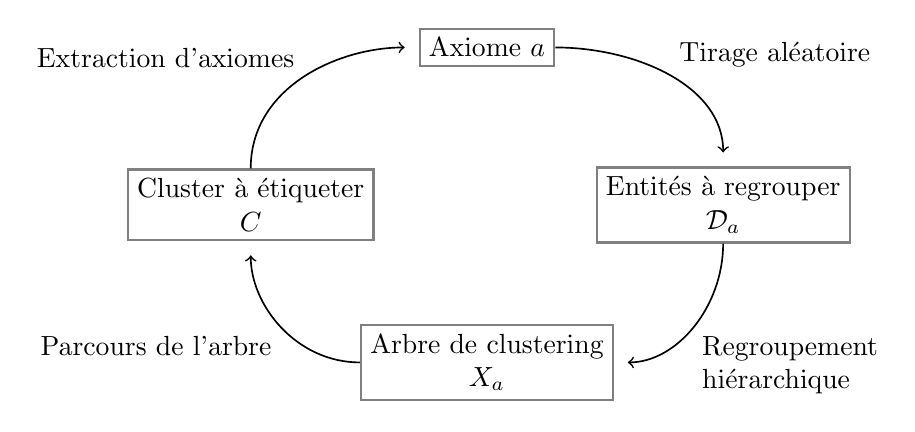
\begin{tikzpicture}[
  box/.style={draw=gray, thick, align=center},
  arrow/.style={->, semithick, shorten >=5pt,}
]
\def\l{2};
\node[box] (s2) at (1.5*\l, 0) {Entités à regrouper \\ $\mathcal{D}_a$};
\node[box] (s1) at (0, \l) {Axiome $a$};
\node[box] (s3) at (0, -\l) {Arbre de clustering \\$X_a$};
\node[box] (s4) at (-1.5*\l, 0) {Cluster à étiqueter \\$C$};

% \textit{Ensemble de $N$ entités vérifiant $a$}

\draw [arrow] (s1) to[out=0, in=90] node[auto] {Tirage aléatoire} (s2);
\draw [arrow] (s2) to[out=270, in=0] node[auto, align=left] {Regroupement \\ hiérarchique} (s3);
\draw [arrow] (s3) to[out=180, in=270]  node[auto] {Parcours de l'arbre}  (s4);
\draw [arrow] (s4) to[out=90, in=180]  node[auto] {Extraction d'axiomes}  (s1);

\end{tikzpicture}